
\begin{enumerate}[label=\thesubsection.\arabic*, ref=\thesubsection.\theenumi]
\item Probability
\begin{itemize}
\item Addition Theorem of Probability:
\begin{align}
P\brak{M} + P\brak{E} - P\brak{ME} + P\brak{\brak{M \cup E}'} = 1 \label{eq:addition_theorem_probability}
\end{align}


\item Complement Laws in Boolean algebra
\begin{align}
	A + A' = 1, \quad AA' = 0 \label{eq:Prob_1}
\end{align}
\item Probability of Certain and Impossible Events
\begin{align}
	P\brak{1} = 1, \quad P\brak{0} = 0 \implies P\brak{A + A'} = 1, \quad P\brak{AA'} = 0 \label{eq:Prob_2}
\end{align}
\item Addition Law of Probability for Mutually Exclusive Events
\begin{align}
	P\brak{A + A'} = P\brak{A} + P\brak{A'} \label{eq:Prob_3}
\end{align}
\item Difference rule of probability
	\begin{align}
{P\brak{AB'} = P\brak{A} - P\brak{AB}}
	\end{align}
\noindent Proof: \\
\noindent Using \eqref{eq:Prob_1}
\begin{align}
A = A \cdot 1 = A\brak{B + B'}
\end{align}
Applying the distributive law:
\begin{align}
A = AB + AB'
\end{align}

\vspace{0.3cm}

\noindent To apply the additive property of probability, we check the intersection of $AB$ and $AB'$:
\begin{align}
\brak{AB}\brak{AB'} = A \cdot A \cdot B \cdot B' = A \cdot \brak{BB'}
\end{align}
Since $BB' = 0$:
\begin{align}
\brak{AB}\brak{AB'} = A \cdot 0 = 0
\end{align}
Thus, the events $AB$ and $AB'$ are mutually exclusive.

\vspace{0.3cm}

\noindent Since $A = AB + AB'$ and $\brak{AB}\brak{AB'} = 0$, from \eqref{eq:Prob_3}
\begin{align}
P\brak{A} = P\brak{AB + AB'} = P\brak{AB} + P\brak{AB'}
\end{align}

\vspace{0.3cm}
\noindent Rearranging the equation (3.9) to isolate $P\brak{AB'}$:
\begin{align}
{P\brak{AB'} = P\brak{A} - P\brak{AB}}
\end{align}

\end{itemize}
\item Laplace Transform
\begin{itemize}
\item Laplace transform on $g'\brak{t}$ \\ \\
\noindent Using the definition of the Laplace transform: 
\begin{align}
\mathcal{L}\{g'\brak{t}\} = \int_{0}^{\infty} e^{-st} g'\brak{t} \, dt
\end{align}

\noindent Applying integration by parts with $u = e^{-st}$ and $dv = g'\brak{t} \, dt$ (giving $du = -s e^{-st} \, dt$ and $v = g\brak{t}$):
\begin{align}
\mathcal{L}\{g'\brak{t}\} &= \left[ e^{-st} g\brak{t} \right]_{0}^{\infty} - \int_{0}^{\infty} \brak{-s e^{-st}} g\brak{t} \, dt \\
&= \left( \lim_{t \to \infty} e^{-st} g\brak{t} - g\brak{0} \right) + s \int_{0}^{\infty} e^{-st} g\brak{t} \, dt 
\end{align}

\noindent 
\begin{align}
\mathcal{L}\{g'\brak{t}\} = 0 - g\brak{0} + s G\brak{s} = s G\brak{s}-g\brak{0} \label{eq:Laplace_1}
\end{align}
\item Laplace transform on $g''\brak{t}$ \\

\noindent Using the definition for $g''\brak{t}$:
\begin{align}
\mathcal{L}\{g''\brak{t}\} = \int_{0}^{\infty} e^{-st} g''\brak{t} \, dt
\end{align}

\noindent Applying integration by parts with $u = e^{-st}$ and $dv = g''\brak{t} \, dt$ (giving $du = -s e^{-st} \, dt$ and $v = g'\brak{t}$):
\begin{align}
\mathcal{L}\{g''\brak{t}\} &= \left[ e^{-st} g'\brak{t} \right]_{0}^{\infty} - \int_{0}^{\infty} \brak{-s e^{-st}} g'\brak{t} \, dt \\
&= \left( \lim_{t \to \infty} e^{-st} g'\brak{t} - g'\brak{0} \right) + s \int_{0}^{\infty} e^{-st} g'\brak{t} \, dt
\end{align}

\noindent With $g'\brak{0} = 0$ and substituting the result from part (a), $\mathcal{L}\{g'\brak{t}\} = s G\brak{s}-g\brak{0}$:
\begin{align} 
\mathcal{L}\{g''\brak{t}\} = 0 - g'\brak{0} + s \brak{s G\brak{s}-g\brak{0}} = s^2 G\brak{s} -sg\brak{0}-g'\brak{0} \label{eq:Laplace_2}
\end{align}

\item The First Frequency Shift Theorem:
\noindent It states that if $\mathcal{L}\{f\brak{x}\} = F\brak{s}$, then:
\begin{align}
\mathcal{L}^{-1}\{F\brak{s - a}\} = e^{ax} f\brak{x} \label{eq:Laplace_3}
\end{align}
\noindent Proof: \\

\noindent 
By definition, the Laplace transform of a function $g\brak{x}$ is:
\begin{align}
\mathcal{L}\{g\brak{x}\} = \int_{0}^{\infty} e^{-sx} g\brak{x} \, dx
\end{align}
\noindent Substituting $g\brak{x} = e^{ax} f\brak{x}$:
\begin{align}
\mathcal{L}\{e^{ax} f\brak{x}\} = \int_{0}^{\infty} e^{-sx} \brak{e^{ax} f\brak{x}} dx
\end{align}

\begin{align}
= \mathcal{L}\{e^{ax} f\brak{x}\} = \int_{0}^{\infty} e^{-\brak{s - a}x} f\brak{x} \, dx
\end{align}


\noindent Recall that $F\brak{s}$ is defined as:
\begin{align}
F\brak{s} = \int_{0}^{\infty} e^{-sx} f\brak{x} \, dx
\end{align}
\noindent Replacing $s$ with $\brak{s - a}$:
\begin{align}
F\brak{s - a} = \int_{0}^{\infty} e^{-\brak{s - a}x} f\brak{x} \, dx
\end{align}
\noindent Therefore:
\begin{align}
\mathcal{L}\{e^{ax} f\brak{x}\} = F\brak{s - a}
\end{align}

\noindent Applying the inverse Laplace operator $\mathcal{L}^{-1}$ to both sides yields:
\begin{align}
\mathcal{L}^{-1}\{F\brak{s - a}\} = e^{ax} f\brak{x}
\end{align}
\item Inverse Laplace Transform on $1/s^2$:
\begin{align}
\mathcal{L}^{-1} \left\{ \frac{1}{s^2} \right\} = x \label{eq:Laplace_4}
\end{align}
\noindent Proof: \\
\begin{align}
\mathcal{L}\brak{x} &= \int_{0}^{\infty} x e^{-sx} \, dx 
\end{align}
\begin{align}
= \brak{-\frac{x}{s}e^{-sx}}_{0}^{\infty} + \frac{1}{s}\int_{0}^{\infty} e^{-sx} \, dx 
\end{align}
\begin{align}
= 0 + \frac{1}{s}\brak{-\frac{1}{s}e^{-sx}}_{0}^{\infty} = \frac{1}{s^2} 
\end{align}
\begin{align}
\implies \mathcal{L}^{-1}\brak{\frac{1}{s^2}} &= x
\end{align}
\item Inverse Laplace Transform to produce the cosine and sine functions
\begin{align}
\mathcal{L}\brak{e^{iax}} &= \int_{0}^{\infty} e^{-sx} e^{iax} \, dx = \int_{0}^{\infty} e^{-(s-ia)x} \, dx \\
&= \brak{-\frac{e^{-(s-ia)x}}{s-ia}}_{0}^{\infty} = \frac{1}{s-ia} \\
&= \frac{s + ia}{(s - ia)(s + ia)} = \frac{s}{s^2 + a^2} + i\frac{a}{s^2 + a^2}
\end{align}

\noindent We know that
\begin{align}
\mathcal{L}\brak{\cos(ax) + i\sin(ax)} = \mathcal{L}\brak{\cos(ax)} + i\,\mathcal{L}\brak{\sin(ax)}:
\end{align}
\noindent Equating the real and imaginary parts, we get:
\begin{align}
	\mathcal{L}\brak{\cos(ax)} &= \frac{s}{s^2 + a^2} \implies \mathcal{L}^{-1}\brak{\frac{s}{s^2 + a^2}} = \cos(ax) \label{eq:Laplace_5}
\end{align}
\begin{align}
	\mathcal{L}\brak{\sin(ax)} &= \frac{a}{s^2 + a^2} \implies \mathcal{L}^{-1}\brak{\frac{a}{s^2 + a^2}} = \sin(ax) \label{eq:Laplace_6}
\end{align}

\item Solving a differential equation of the form:
\begin{align}
	\frac{d^2 y}{d x^2}= -\alpha^2 y, \alpha \neq 0
\end{align}
\noindent Applying the Laplace Transform on both sides, and using \eqref{eq:Laplace_2}, we get:
\begin{align}
	s^2G(s)-sy(0)-y'(0)=-\alpha^2 G(s)
\end{align}
\noindent Let $y(0) = \beta$ and $y'(0)= \gamma$ \\
\noindent Rearranging, we get:
\begin{align}
G(s)=\frac{s\beta + \gamma}{s^2 + \alpha^2}
\end{align}
\begin{align}
G(s)=\frac{s\beta}{s^2 + \alpha^2}+\frac{\gamma}{s^2 + \alpha^2}
\end{align}
\noindent From results \eqref{eq:Laplace_5} and \eqref{eq:Laplace_6}, we get:
\begin{align}
	G(s)=\beta cos(\alpha x) + \frac{\gamma}{\alpha}sin(\alpha x) \label{eq:Laplace_7}
\end{align}
\end{itemize}
\item Euler's Method of Forward Differences
\begin{itemize}
	\item First Forward Difference: \\
		\noindent Consider a differential equation:
\begin{align}
	\frac{dy}{dx}=f\brak{x,y}, y\brak{x_0}=y_0
\end{align}
\noindent The slope of the tangent $m$ at $x=x_0$ is given by:
\begin{align}
m=f\brak{x_0,y_0}
\end{align}
		\noindent The slope of the tangent line gives the direction in which we need to move in order to trace the curve(considering we move in small steps). Hence, we can numerically compute the approximate value of a function at a given $x$ knowing the initial conditions. \\
\begin{figure}[H]
\begin{center}
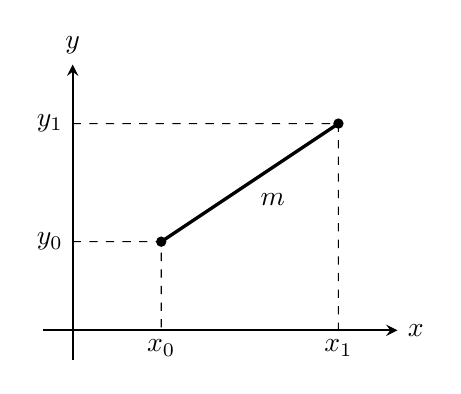
\begin{tikzpicture}[scale=0.75]
    % Axes
    \draw[->, >=stealth, thick] (-0.5, 0) -- (5.5, 0) node[right] {$x$};
    \draw[->, >=stealth, thick] (0, -0.5) -- (0, 4.5) node[above] {$y$};

    % Define Point Coordinates
    \coordinate (P0) at (1.5, 1.5);
    \coordinate (P1) at (4.5, 3.5);

    % Dashed reference lines to axes
    \draw[dashed] (0, 1.5) node[left] {$y_0$} -- (P0) -- (1.5, 0) node[below] {$x_0$};
    \draw[dashed] (0, 3.5) node[left] {$y_1$} -- (P1) -- (4.5, 0) node[below] {$x_1$};

    % Solid line connecting points with slope 'm'
    \draw[very thick] (P0) -- (P1) node[midway, below right] {$m$};

    % Data point markers
    \fill (P0) circle (2.5pt);
    \fill (P1) circle (2.5pt);
\end{tikzpicture}
\makeatletter
    \long\def\@makecaption#1#2{%
      \vskip\abovecaptionskip
      \begin{center}
        #1 #2
      \end{center}
      \vskip\belowcaptionskip}
    \makeatother
    \caption{Zoomed in graph}
    \label{fig:1}

\end{center}
\end{figure}
\noindent Consider the above diagram, the equation of line is:
\begin{align}
	y_1-y_0=m\brak{x_1-x_0}
\end{align}
\begin{align}
y_1=y_0+mh
\end{align}
\noindent Here, $h=x_1-x_0$ is the step size(or small increment in $x$) \\
\noindent Generalising the above result, we get the derivative $y'_n$:
\begin{align}
	y'_n=\frac{y_{n+1}-y_n}{h} \label{eq:ED_1}
\end{align}
\item Second Forward Difference: \\ \\
	\noindent Differentiating the equation \eqref{eq:ED_1}, we obtain:
\begin{align}
	y_n''=\frac{y_{n+1}'-y_n'}{h}
\end{align}
		\noindent From equation \eqref{eq:ED_1}, we obtain:
		\begin{align}
			y_{n+1}'=\frac{y_{n+2}-y_{n+1}}{h} &, y_n'=\frac{y_{n+1}-y_n}{h}
		\end{align}
\noindent Substituting, we get: 
\begin{align}
	y_n''=\frac{y_{n+2}-2y_{n+1}+y_n}{h^2} \label{eq:ED_2}
\end{align}


\end{itemize}
\item The Fourier Series \\
\noindent Any continuous or piecewise-continuous periodic function can be expressed as an infinite sum of complex exponentials.
\begin{align}
x\brak{t} &= \sum_{k=-\infty}^{\infty} c_k e^{j 2\pi k f_0 t} 
\end{align}
\noindent Multiply both sides by $e^{-j2\pi m f_0 t}$ (where $m$ is an integer) and integrate over the interval
$\left[-\frac{1}{2f_0}, \frac{1}{2f_0}\right]$
\begin{align}
\int_{-\frac{1}{2f_0}}^{\frac{1}{2f_0}} x\brak{t} e^{-j 2\pi m f_0 t} \, dt
\end{align}
\begin{align}
= \int_{-\frac{1}{2f_0}}^{\frac{1}{2f_0}} \brak{\sum_{k=-\infty}^{\infty} c_k e^{j 2\pi k f_0 t}} e^{-j 2\pi m f_0 t} \, dt 
\end{align}
\begin{align}
=\sum_{k=-\infty}^{\infty} c_k \int_{-\frac{1}{2f_0}}^{\frac{1}{2f_0}} e^{j 2\pi \brak{k - m} f_0 t} \, dt
\end{align}

Using the orthogonality property over the period $T_0 = \frac{1}{f_0}$:
\begin{align}
\int_{-\frac{1}{2f_0}}^{\frac{1}{2f_0}} e^{j 2\pi \brak{k - m} f_0 t} \, dt &= 
\begin{cases} 
\frac{1}{f_0}, & k = m \\ 
0, & k \neq m 
\end{cases} \notag
\end{align}

Substituting this back into the sum isolates the term for $k = m$:
\begin{align}
\int_{-\frac{1}{2f_0}}^{\frac{1}{2f_0}} x\brak{t} e^{-j 2\pi m f_0 t} \, dt &= c_m \cdot \frac{1}{f_0} 
\end{align}
\begin{align}
	c_k &= f_0 \int_{-\frac{1}{2f_0}}^{\frac{1}{2f_0}} x\brak{t} e^{-j 2\pi k f_0 t} \, dt \label{eq:Fourier_1}
\end{align}

\item Matrices
\begin{itemize}
	\item Fundamental property: 
	\begin{align}
	\mydet{\mathbf{A^T}} = \mydet{\mathbf{A}} \label{eq:Matrices_1} 
	\end{align}
	\noindent Proof: \\
	 \noindent When expanding $\mydet{\mathbf{A}}$ along Row 1, you select entries across the top row and compute the determinants of their remaining submatrices.

\noindent When expanding $\mydet{\mathbf{A^T}}$ down Column 1, those exact same entries now sit vertically in the first column, and their corresponding submatrices are simply transposed.


\noindent Visual Matrix Comparison:

\noindent
Matrix $\mathbf{A}$ (Expand along Row 1):
\begin{align}
\mydet{\mathbf{A}} = 
\begin{vmatrix}
\mathbf{a_{11}} & \mathbf{a_{12}} & \mathbf{a_{13}} \\
a_{21} & a_{22} & a_{23} \\
a_{31} & a_{32} & a_{33}
\end{vmatrix}
\end{align}

\noindent
Matrix $\mathbf{A^T}$ (Expand down Column 1):
\begin{align}
\mydet{\mathbf{A^T}} = 
\begin{vmatrix}
\mathbf{a_{11}} & a_{21} & a_{31} \\
\mathbf{a_{12}} & a_{22} & a_{32} \\
\mathbf{a_{13}} & a_{23} & a_{33}
\end{vmatrix}
\end{align}

\noindent  Submatrix Comparison for Entry $a_{12}$:\\

When selecting $a_{12}$:
\begin{itemize}
    \item In $\mathbf{A}$ (Row 1, Column 2 deletion):
    \begin{align}
    \mathbf{M_{12}} = \myvec{ a_{21} & a_{23} \\ a_{31} & a_{33} }
    \end{align}

    \item In $\mathbf{A^T}$ (Row 2, Column 1 deletion):
    \begin{align}
    \mathbf{N_{21}} = \myvec{ a_{21} & a_{31} \\ a_{23} & a_{33} }
    \end{align}
\end{itemize}

\noindent Notice that $\mathbf{N_{21}} = \brak{\mathbf{M_{12}}}^T$. Since $\mydet{\mathbf{M_{12}}} = \mydet{\brak{\mathbf{M_{12}}}^T}$, every term in the expansion of $\mydet{\mathbf{A}}$ is identically equal to the corresponding term in $\mydet{\mathbf{A^T}}$. \\
\item A few relations on the eigenvalues of a matrix \\
	\noindent Let $\lambda_1, \lambda_2, .... , \lambda_i$ be the eigenvalues of a matrix $\mathbf{A}$. Then, we have:
\begin{align}
	\sum_{i=1}^{n} \lambda_i = \text{Tr}\brak{\mathbf{A}} \label{eq:Matrices_2}
\end{align}
\begin{align}
	\prod_{i=1}^{n} \lambda_1 = \mydet{\mathbf{A}} \label{eq:Matrices_3}
\end{align}
\item Results on the conic sections
\begin{enumerate}
\item
The equation of  a conic with directrix $\vec{n}^{\top}\vec{x} = c$, eccentricity $e$ and focus $\vec{F}$ is given by 
\begin{align}
    \label{eq:app-conic_quad_form}
	\text{g}\brak{\vec{x}} = \vec{x}^{\top}\vec{V}\vec{x}+2\vec{u}^{\top}\vec{x}+f=0
    \end{align}
where     
\begin{align}
  \label{eq:app-conic_quad_form_v}
\vec{V} &=\norm{\vec{n}}^2\vec{I}-e^2\vec{n}\vec{n}^{\top}, 
\\
\label{eq:app-conic_quad_form_u}
\vec{u} &= ce^2\vec{n}-\norm{\vec{n}}^2\vec{F}, 
\\
\label{eq:app-conic_quad_form_f}
f &= \norm{\vec{n}}^2\norm{\vec{F}}^2-c^2e^2
    \end{align}
\noindent Proof:
\begin{align}
\|\mathbf{x} - \mathbf{F}\|^2 &= e^2 \frac{(\mathbf{n}^\top \mathbf{x} - c)^2}{\|\mathbf{n}\|^2} 
\end{align}
\begin{align}
\implies \|\mathbf{n}\|^2 (\mathbf{x} - \mathbf{F})^\top (\mathbf{x} - \mathbf{F}) &= e^2 \left(\mathbf{n}^\top \mathbf{x} - c\right)^2 
\end{align}
\begin{align}
\implies \|\mathbf{n}\|^2 \left(\mathbf{x}^\top \mathbf{x} - 2\mathbf{F}^\top \mathbf{x} + \|\mathbf{F}\|^2\right) &= e^2 \left(c^2 + \left(\mathbf{n}^\top \mathbf{x}\right)^2 - 2c\mathbf{n}^\top \mathbf{x}\right) 
\end{align}
\begin{align}
= e^2 \left(c^2 + \left(\mathbf{x}^\top \mathbf{n}\mathbf{n}^\top \mathbf{x}\right) - 2c\mathbf{n}^\top \mathbf{x}\right)
\end{align}
		\noindent which can be expressed as \eqref{eq:app-conic_quad_form} after simplification.
\item
  The eccentricity of \eqref{eq:app-conic_quad_form} is given by 
\begin{align}
  \label{eq:app-conic_quad_form_e} 
  e&= \sqrt{1-\frac{\lambda_1}{\lambda_2}}
\end{align} 
		Here, $\lambda_1$ and $\lambda_2$ are the eigenvalues of $\mathbf{V}$ \\
	\label{app:conic-parameters}
\noindent Proof: \\
\noindent From \eqref{eq:app-conic_quad_form_v}, using the fact that $\vec{V}$ is symmetric with $\vec{V} = \vec{V}^{\top}$,
  \begin{align}
	  \vec{V}^{\top} \vec{V}&=\brak{\norm{\vec{n}}^2\vec{I}-e^2\vec{n}\vec{n}^{\top}}^{\top}
	  \brak{\norm{\vec{n}}^2\vec{I}-e^2\vec{n}\vec{n}^{\top}}
    \\
	  \implies \vec{V}^{2} &= \norm{\vec{n}}^4\vec{I}+e^4\vec{n}\vec{n}^{\top}\vec{n}\vec{n}^{\top}
	  -2e^2\norm{\vec{n}}^2\vec{n}\vec{n}^{\top}
    \\
	  &= \norm{\vec{n}}^4\vec{I} + e^4\norm{\vec{n}}^2\vec{n}\vec{n}^{\top}
	%  \\
	  - 2e^2\norm{\vec{n}}^2\vec{n}\vec{n}^{\top}
    \\
	  &= \norm{\vec{n}}^4\vec{I} + e^2\brak{e^2 - 2}\norm{\vec{n}}^2\vec{n}\vec{n}^{\top}
    \\
	  &= \norm{\vec{n}}^4\vec{I} + \brak{e^2 - 2}\norm{\vec{n}}^2\brak{\norm{\vec{n}}^2\vec{I}- \vec{V}}
    \end{align}
%    
which can be expressed as
\begin{align}
  \vec{V}^{2} + \brak{e^2 - 2}\norm{\vec{n}}^2\vec{V} - \brak{e^2 - 1}\norm{\vec{n}}^4\vec{I}=0
  \label{eq:app-conic_quad_form_e_cayley}
\end{align}
	Using the Cayley-Hamilton theorem,
	\eqref{eq:app-conic_quad_form_e_cayley} results in the characteristic equation, 
\begin{align}
  \lambda^{2} - \brak{2-e^2}\norm{\vec{n}}^2\lambda + \brak{1-e^2 }\norm{\vec{n}}^4=0
\end{align}
which can be expressed as
\begin{align}
\brak{\frac{\lambda}{\norm{\vec{n}}^2}}^2 - \brak{2-e^2 }\brak{\frac{\lambda}{\norm{\vec{n}}^2}} 
	+ \brak{1-e^2 } = 0
	\\
	\implies \frac{\lambda}{\norm{\vec{n}}^2} = 1-e^2, 1
  \\
	\text{or, }\lambda_2 = \norm{\vec{n}}^2, \lambda_1 = \brak{1-e^2}\lambda_2 
  \label{eq:app-conic_quad_form_lam_cayley}
\end{align}
\item
\eqref{eq:app-conic_quad_form} represents 
	\begin{enumerate}
		\item a parabola for $\mydet{\vec{V}} = 0 $,
		\item ellipse for $\mydet{\vec{V}} > 0 $ and 
		\item hyperbola for $\mydet{\vec{V}} < 0 $. \label{item:Hyperbola}
	\end{enumerate}
\noindent This is a direct result of the following two equations: \\
\noindent From \eqref{eq:app-conic_quad_form_e}, we have
\begin{align}
\frac{\lambda_1}{\lambda_2}=1-e^2
\end{align}
\noindent From \eqref{eq:Matrices_3}, we have
\begin{align}
\mydet{\mathbf{V}}=\lambda_1 \lambda_2
\end{align}
\end{enumerate}
\item Matrix Determinant Lemma \\
\noindent Consider two column vectors $\mathbf{u} and \mathbf{v}$
\begin{align}
	\mydet{\mathbf{I+uv^T}}=1+\mathbf{v^Tu}	\label{eq:mat_det_lemma}
\end{align}
\end{itemize}
\end{enumerate}
\clearpage
